\section{Experiments}

\subsection{Experimental Setup}

\paragraph{Models.}
本文比较 RoBERTa 微调模型与 4 个本地 Qwen 小模型：Qwen3-0.6B、Qwen3-1.7B、Qwen3.5-0.8B 和 Qwen3.5-2B。所有 LLM 实验均在同一份 \comve Task A test 集上运行，并分别测试 no-thinking 与 thinking 两种推理模式。Task B 在相同模型集合上进一步评估 direct prompting、constraint-first prompting 与 generate-verify-rerank 三种 test-time enhancement 策略。

\paragraph{Prompts and outputs.}
Task A 使用 direct、judge 和 minimal 三种 prompt 模板；8-shot 设置在同一测试集上加入 8 个固定训练示例；self-consistency 设置对每个样本和模板重复采样 5 次并做多数投票。实验使用项目内固定测试集，共 1,000 条样本。Task B 在同一测试集上复用 direct baseline，并额外比较 constraint-first 与 generate-verify-rerank。两个方向的输出都写入项目的 results 目录；报告正文只引用汇总指标，复现入口和文件组织放在附录说明。

\paragraph{Metrics.}
主实验报告 accuracy；鲁棒性实验报告 order consistency、prompt consistency 和 sampling consistency。Order consistency 衡量交换两个候选句顺序后模型预测是否同步翻转；prompt consistency 衡量同一模型在三种模板下预测是否一致；sampling consistency 衡量重复采样的多数标签占比。Task B 报告不同推理增强策略的最终 accuracy，并用折线图比较模型规模与推理模式的关系。

\paragraph{Completeness check.}
Task A vLLM 实验覆盖 zero-shot、8-shot、order swap 和 self-consistency；Task B 实验覆盖 direct、constraint-first 和 rerank。两部分都以同一测试集大小作为基本校验，预测文件和指标文件均通过行数检查。

\subsection{Task A Main Results}

\begin{table}[t]
\centering
\small
\resizebox{\linewidth}{!}{%
\begin{tabular}{lccc}
\toprule
Method & Acc. & Consistency & Notes \\
\midrule
RoBERTa fine-tuning & 0.868 & Order 0.939 & supervised \\
Qwen3-1.7B zero-shot & \textbf{0.952} & Prompt 0.849 / Order 0.929 & thinking, direct \\
Qwen3-1.7B 8-shot & 0.931 & Prompt 0.849 & thinking, direct \\
Qwen3.5-2B self-consistency & 0.720 & Prompt 0.550 / Sampling 0.794 & no-thinking, minimal \\
\bottomrule
\end{tabular}%
}
\caption{\comve Task A 主结果。Acc. 为测试集准确率；Consistency 列报告该设置下最相关的一致性指标。}
\label{tab:main_results}
\end{table}

表~\ref{tab:main_results} 显示，最佳 LLM 设置显著超过 RoBERTa：Qwen3-1.7B thinking zero-shot direct prompt 达到 0.952 准确率，比 RoBERTa 高 8.4 个百分点。同时，该设置的 order consistency 为 0.929，接近 RoBERTa 的 0.939，说明高准确率并非完全来自位置偏置。8-shot 没有提升最佳 direct prompt，反而从 0.952 降至 0.931。No-thinking self-consistency 的最佳结果为 Qwen3.5-2B minimal prompt，准确率 0.720，低于 thinking zero-shot，但高于同模型 no-thinking zero-shot minimal prompt 的 0.684。

\subsection{Task A Zero-shot Results}

本小节单独展开 zero-shot，是因为它构成后续 few-shot、self-consistency 与 Task B direct baseline 的参照点。表~\ref{tab:zero_results} 汇总每个代表模型和推理模式下的最佳 prompt，可以看到 thinking 模式在所有强模型上都明显占优；no-thinking 设置虽然偶尔能通过 minimal prompt 获得可用结果，但整体上仍低于对应 thinking 版本。

\begin{table}[t]
\centering
\small
\resizebox{\linewidth}{!}{%
\begin{tabular}{llcc}
\toprule
Model & Setting & Best prompt & Acc. \\
\midrule
Qwen3-1.7B & thinking & direct & \textbf{0.952} \\
Qwen3-0.6B & thinking & minimal & 0.819 \\
Qwen3.5-2B & thinking & direct & 0.803 \\
Qwen3.5-0.8B & thinking & direct & 0.724 \\
Qwen3-1.7B & no-thinking & minimal & 0.706 \\
Qwen3.5-2B & no-thinking & minimal & 0.684 \\
\bottomrule
\end{tabular}%
}
\caption{Zero-shot 设置下每个代表模型/模式的最佳 prompt。Thinking 模式整体优于 no-thinking。}
\label{tab:zero_results}
\end{table}

从 prompt 角度看，direct prompt 对 Qwen3-1.7B 和 Qwen3.5-2B thinking 最有效，而 minimal prompt 对 Qwen3-0.6B thinking 与 no-thinking 模型更稳。这说明不同规模模型对指令复杂度的偏好并不相同：较强模型能够利用更明确的判断指令，较弱模型则更容易从短 prompt 中受益。这个观察也解释了为什么后续 Task B 不只比较最终 accuracy，还需要比较 direct、constraint-first 和 rerank 三种推理形式。

\subsection{Task A Robustness Results}

\begin{table}[t]
\centering
\small
\resizebox{\linewidth}{!}{%
\begin{tabular}{lcccc}
\toprule
Method & Acc. & Swap Acc. & Order & Prompt \\
\midrule
RoBERTa fine-tuning & 0.868 & 0.867 & \textbf{0.939} & -- \\
Qwen3-1.7B thinking direct & \textbf{0.952} & \textbf{0.949} & 0.929 & \textbf{0.849} \\
Qwen3-1.7B thinking judge & 0.938 & 0.932 & 0.908 & \textbf{0.849} \\
Qwen3-1.7B thinking minimal & 0.885 & 0.888 & 0.811 & \textbf{0.849} \\
Qwen3.5-2B thinking direct & 0.803 & 0.784 & 0.691 & 0.461 \\
Qwen3.5-2B thinking minimal & 0.800 & 0.786 & 0.676 & 0.461 \\
\bottomrule
\end{tabular}%
}
\caption{顺序交换与提示一致性结果。Swap Acc. 是交换句子顺序后的准确率；Order 是原始预测与交换预测是否同步翻转。}
\label{tab:robustness_results}
\end{table}

表~\ref{tab:robustness_results} 中，Qwen3-1.7B thinking 不仅准确率最高，而且在三种 prompt 上都保持较高顺序一致性。相比之下，Qwen3.5-2B thinking 的准确率仍可达到 0.800 左右，但 order consistency 降至 0.676--0.691，说明它对句子位置和 prompt 形式更敏感。若再看 sampling consistency，Qwen3-1.7B thinking 的多数标签占比为 0.888，明显高于对应 no-thinking 设置，说明其多次采样时的决策边界也更稳定。

\subsection{Few-shot and Self-consistency}

\begin{table}[t]
\centering
\small
\resizebox{\linewidth}{!}{%
\begin{tabular}{llccc}
\toprule
Model & Prompt & Zero-shot & 8-shot & Delta \\
\midrule
Qwen3-1.7B thinking & direct & 0.952 & 0.931 & -0.021 \\
Qwen3-1.7B thinking & judge & 0.938 & 0.920 & -0.018 \\
Qwen3-1.7B thinking & minimal & 0.885 & 0.891 & +0.006 \\
Qwen3.5-2B thinking & direct & 0.803 & 0.500 & -0.303 \\
Qwen3-0.6B thinking & minimal & 0.819 & 0.607 & -0.212 \\
\bottomrule
\end{tabular}%
}
\caption{8-shot 与 zero-shot 的比较。少样本示例并未稳定提升，部分模型明显退化。}
\label{tab:fewshot_results}
\end{table}

\begin{table}[t]
\centering
\small
\resizebox{\linewidth}{!}{%
\begin{tabular}{llccc}
\toprule
Model & Prompt & Acc. & Prompt & Sampling \\
\midrule
Qwen3.5-2B no-thinking & minimal & \textbf{0.720} & 0.550 & 0.794 \\
Qwen3-1.7B no-thinking & minimal & 0.701 & 0.252 & \textbf{0.970} \\
Qwen3.5-2B no-thinking & direct & 0.568 & 0.550 & 0.767 \\
Qwen3-1.7B no-thinking & direct & 0.563 & 0.252 & 0.967 \\
\bottomrule
\end{tabular}%
}
\caption{No-thinking self-consistency，采样次数 $k=5$。Sampling 是多数标签占比的平均值。}
\label{tab:self_consistency_results}
\end{table}

表~\ref{tab:self_consistency_results} 表明，采样一致性不能直接等同于正确性。Qwen3-1.7B no-thinking minimal prompt 的 sampling consistency 高达 0.970，但准确率只有 0.701；Qwen3.5-2B no-thinking minimal prompt 的采样一致性较低，却获得更高准确率 0.720。

\subsection{Task B Main Results}

Task B 的目标不是重新设计数据集，而是在 Task A 的二分类常识验证框架上测试推理时增强是否有额外收益。因此表~\ref{tab:verification_results} 采用与 Task A 主表相同的读法：先看 direct baseline，再比较增强策略相对 direct 的变化。Task B direct 与 Task A direct 基本处于同一数量级，说明两个方向在输出约束对齐后具有可比性。

\begin{table*}[t]
\centering
\small
\setlength{\tabcolsep}{4.5pt}
\begin{tabular}{llrrrr}
\toprule
Model & Mode & Task A Direct & Task B Direct & Constraint & Rerank \\
\midrule
Qwen3-0.6B & no-think & 0.500 & 0.500 & 0.500 & 0.434 \\
Qwen3-1.7B & no-think & 0.565 & 0.574 & 0.504 & 0.737 \\
Qwen3.5-0.8B & no-think & 0.470 & 0.466 & 0.478 & 0.500 \\
Qwen3.5-2B & no-think & 0.566 & 0.572 & 0.560 & 0.602 \\
Qwen3-0.6B & think & 0.709 & 0.682 & 0.694 & 0.712 \\
Qwen3-1.7B & think & 0.952 & 0.941 & 0.946 & 0.950 \\
Qwen3.5-0.8B & think & 0.724 & 0.691 & 0.703 & 0.721 \\
Qwen3.5-2B & think & 0.803 & 0.782 & 0.795 & 0.818 \\
\bottomrule
\end{tabular}
\caption{Task B 主结果。Task A Direct 是同模型 direct prompt 的参照基线；其余三列为 Task B 中的 direct、constraint-first 和 generate-verify-rerank。}
\label{tab:verification_results}
\end{table*}

表~\ref{tab:verification_results} 中的整体排序与 Task A 保持一致：Qwen3-1.7B thinking 仍然最强，Qwen3.5-2B thinking 次之，小模型和 no-thinking 设置明显更不稳定。这种一致性很重要，因为它说明 Task B 的增强流程没有引入一个完全不同的评估问题，而是在同一常识验证能力上观察 test-time inference 的边际收益。

\subsection{Task B Strategy Comparison}

从策略对比看，constraint-first 的收益依赖模型是否具备足够稳定的中间推理能力。在 thinking 模式下，它通常略高于 direct，例如 Qwen3-1.7B 从 0.941 提升到 0.946，Qwen3.5-2B 从 0.782 提升到 0.795；但在 no-thinking 模式下，constraint-first 对小模型帮助有限，甚至可能因为中间链条更长而扩大错误传播。

Generate-verify-rerank 的作用更接近对候选解释的筛选。强模型 direct 阶段已经能做出较优判断，因此 rerank 的提升较小但方向稳定；中强模型的收益更明显，例如 Qwen3.5-2B thinking 从 constraint-first 的 0.795 进一步提升到 0.818。相反，对于基础推理能力不足的模型，候选生成本身质量不稳定，verifier 能筛出的有效信息有限。

\subsection{Task B Figure Analysis}

\begin{figure}[t]
\centering
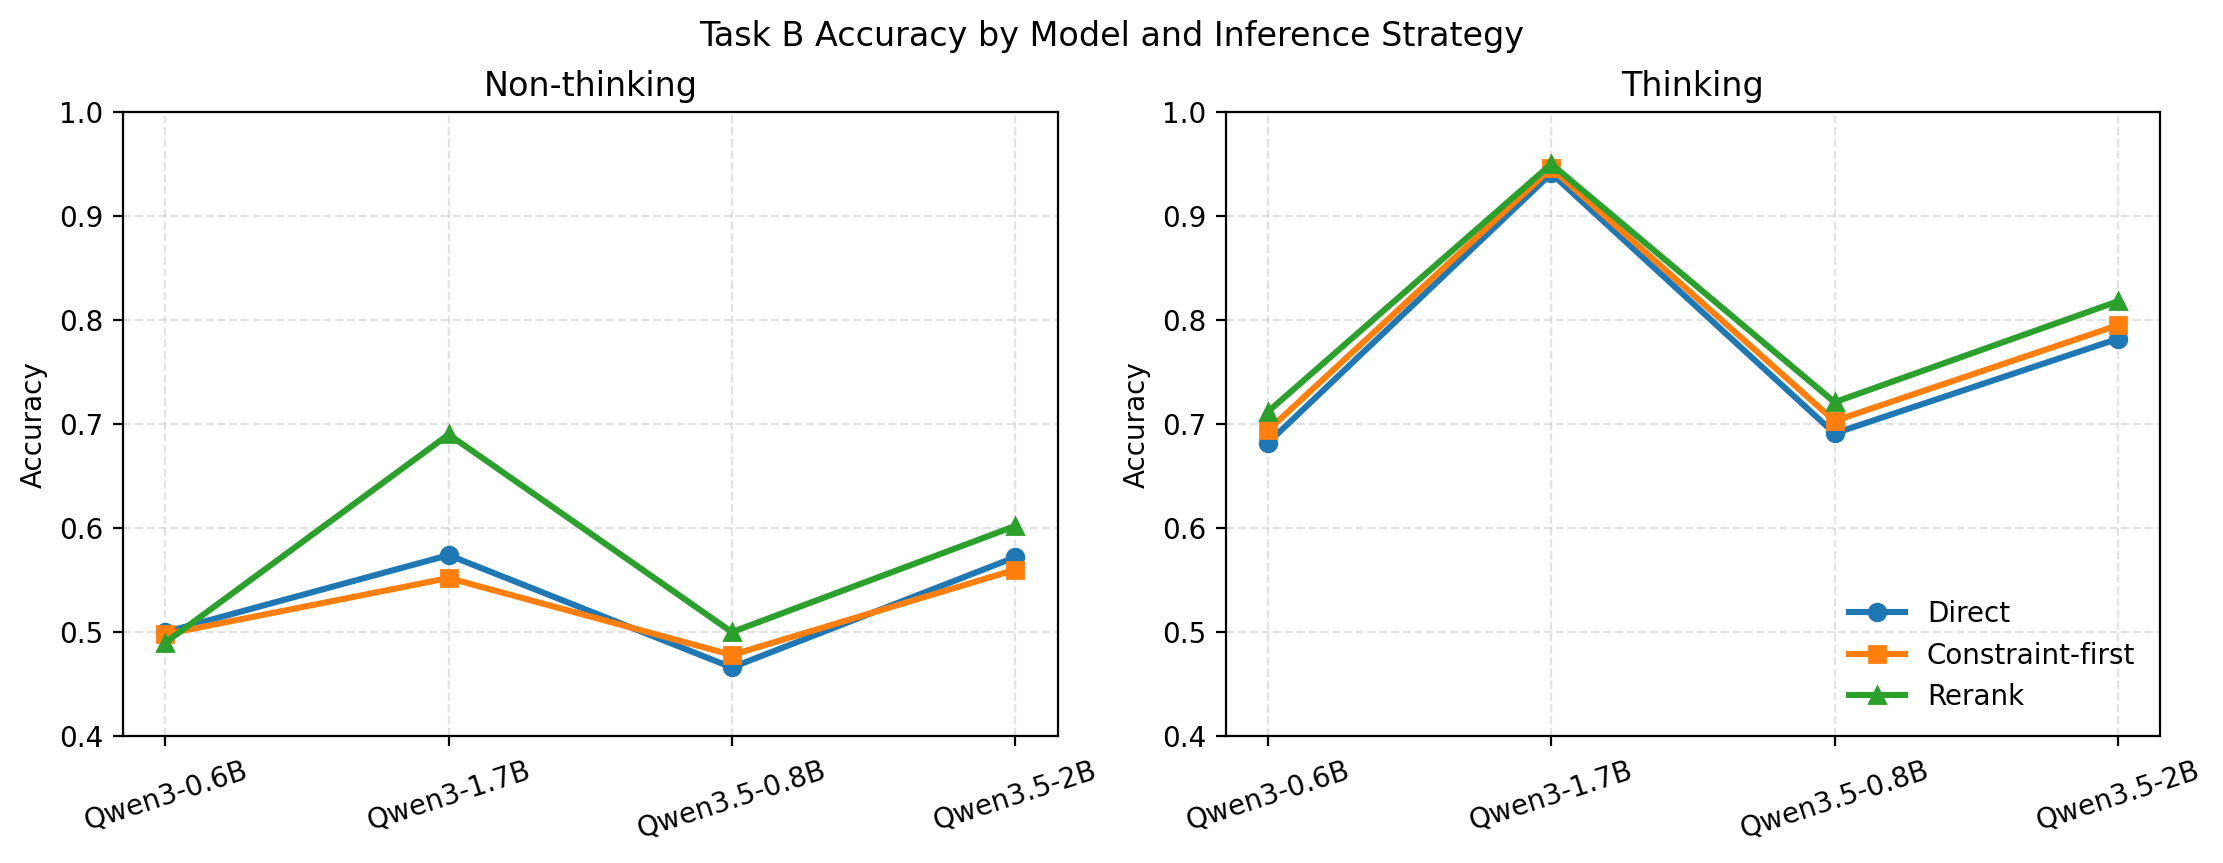
\includegraphics[width=\linewidth]{figures/task_b_accuracy_lines.png}
\caption{Task B 中不同推理策略随模型规模变化的准确率折线图。左图为 no-thinking，右图为 thinking。可以看到 thinking 模式下三条曲线整体上移，而 rerank 曲线在 stronger models 上与其他方法拉开更明显差距。}
\label{fig:taskb_accuracy_lines}
\end{figure}

图~\ref{fig:taskb_accuracy_lines} 将表格中的趋势可视化。左侧 no-thinking 曲线波动较大，说明在基础推理不稳定时，增加 constraint 或 verifier 不一定可靠；右侧 thinking 曲线整体上移，并且 direct、constraint、rerank 的相对顺序更清晰。由此可以把 Task B 的结论概括为：推理时增强更像能力放大器，而不是能力替代器；它最适合已经具备较强常识判断能力、但仍会在边界样本上摇摆的模型。
